\documentclass[a4paper]{article}
\usepackage[utf8]{inputenc}
\usepackage[english]{babel}
\usepackage{biblatex}
\usepackage{graphicx}
\usepackage{float}
% \usepackage{amsmath}
\usepackage{hyperref}
\hypersetup{
    colorlinks,
%     citecolor=black,
    % filecolor=black
    linkcolor=blue,
%     urlcolor=black
}

\addbibresource{sample.bib}




\title{
Using Random Fourier Features with \\ Random Forests \\
\large Deliverable 2: Project Planning}
\author{Albert Ribes Marzá}
\date{March 12, 2018}


\begin{document}
    \maketitle
    \pagebreak

    \tableofcontents
    \pagebreak

    \section{Project Planning}

    The estimated project duration is about 4 months. The project starts on Thursday \(1^{st}\) of February, 2018 and the deadline is on Monday \(18^{th}\) June, 2018.

    As a disclaimer, it must be pointed out that the initial planning could be revised and updated as a result of the evolution of the project.

    % \begin{itemize}
    %     \item El tiempo estimado del proyecto
    %     \item Cuando tengo que entregar el proyecto
    %     \item Avisar que quizá tengo que modificar el planning inicial
    % \end{itemize}

    \section{Plan description}

    The whole project can be divided in 3 different sections. On the first one, Theoretical approach, I will focus on the study field in order to get a better understanding of the issues about mixing Random Forests with Random Fourier Features. On the second section, Algorithm Implementation, I will use the conclusions reached on the first one in order to implement the machine learning algorithm. Finally, in Testing, I will compare the performance of the current Random Forest algorithm with the implemented one, both in accuracy of results and in running time.

    It must be noted after the Testing section, depending on the results obtained, it is possible that a little bit more of work in the other sections may be needed, if there is a real believe that it can be improved with the extra effort. This work is not explained in the following sections, but it is planned to be done after the testing section.

    In addition, the composition of the final document for the project is an important part, but it is not included in the 3 sections described above.

        \subsection{Theoretical approach}

        This section doesn't require special tools to be achieved, but it can be divided in several subsections, apart from a general understanding of the fields of the project:

        \subsubsection{What kernel function should I choose to approximate?}

        The Random Fourier Features extraction core idea is to produce a mapping of the original features of the data which is an approximation of a shift-invariant kernel function. This feature space is the one we are going to use to feed the Random Forest to build a good classifier.

        Hence, we have to decide what is a good kernel function to be approximated.

        \subsubsection{What is the suitable dimensionality of the new feature space derived from the mapping?}

        The number of features in the new space doesn't need to be the same as in the original space. It can be much lower, which can be good to improve the training speed.

        It must be decided what is the best dimensionality to feed the Random Forest.

        \subsubsection{What changes should be made to the original algorithm in order in order to correctly handle the new mapping of the features?}

        The original Random Forest Algorithm is not designed to be used the way we want, so we will have to decide what changes are needed to be made in order to get good results. Some of the decisions we will have to make will be: will we feed the trees in the forest with the same mappings, or with a random subset of it, or with different mappings on the same data?; or: will we need to change the splitting conditions of the nodes in the trees?


        %
        % \begin{itemize}
        %     \item Qué funciones kernel debo usar
        %     \item Detalles sobre cómo modificar los random forest para que todo cuadre
        %     \item La dimensión de los datos del mapping que debo usar
        % \end{itemize}
        \subsection{Algorithm implementation}

        The implementation of the algorithm will be made using the Python 3 programming language. To do so I will need a computer, the source code of the scikit-learn tools together with the documentation and some machine learning and maths modules from Python 3. Several things will have to be done:

        \subsubsection{Implement the random mapping of the data using the Fourier Features algorithm}

        This is just a simple module to map the original feature space to the new one.

        \subsubsection{Get familiar with Scikit Random Forest Classifier module}

        This is strictly not implementation, but it is needed to proceed with the modification. I need to know how is the architecture of the original module in order to write the modifications and join them with the rest of the code.

        \subsubsection{Modify the Scikit module to work with the new features}

        Just as the title says. It is expected that most of the original code will be used and I will only need to modify a tiny fraction.

        \subsubsection{Debug the code}

        It is very likely that I will find bugs is my code, so I will have to fix it. It may take up an important amount of the algorithm implementation.



        %
        % \begin{itemize}
        %     \item El método que transforma los datos de entrada en los nuevos datos
        %     \item Familiarizarme con el módulo de sklearn
        %     \item Modificación del algoritmo que ya está hecho
        % \end{itemize}
        \subsection{Testing}

        This is an essential part of the project. After everything is done, we need to check if the modifications done to the algorithm help to improve the performance. The tools needed in this section are datasets, the code from the previous section and the computer. This section needs the following tasks:

        \subsubsection{Look up suitable testing datasets}

        A real problem dataset is preferred for this testing, specially a dataset which which has been previously used for algorithm testing purposes.

        The dataset should be for a classification problem, and it is important to have a big number of instances, since the algorithm is intended to work and very big problems.

        If it is not possible to find a suitable datasets, I can build it from dummy data.

        \subsubsection{Preprocess the testing datasets if needed}

        If the dataset is not in good conditions (number of missing or unknown values, abnormal values, etc.) I will have to preprocess it in order to fit the needs of the algorithm.

        \subsubsection{Carry out accuracy tests}

        Just as asserted. A suitable metric will be used depending on the found dataset and the kind of problem.

        \subsubsection{Carry out timing tests}

        Forgetting about the accuracy obtained (but assuming it is not too bad), it will be evaluated the time needed to successfully train the model, just to see if it is faster than currently used algorithms.

        \subsubsection{Study the results of the testing}

        The point of all the project is to check if the suggested method performs well on several problems, so the results of the test will be studied to give an answer to the project.




        %
        % \begin{itemize}
        %     \item Buscarme datasets para hacer las pruebas
        %     \item Hacer el preprocessing adecuado
        %     \item Ejecutar test de resultados
        %     \item Ejecutar test de tiempo
        % \end{itemize}



    \section{Estimated Time}

    \begin{center}
    \begin{tabular}{|c|c|}

        \hline
        \textbf{Task} & \textbf{Estimated duration (h)} \\
        \hline \hline
        Background approximation & 50 \\
        Decide the kernel & 6 \\
        Decide dimensionality & 4 \\
        Decide the changes & 10 \\
        \hline
        \textbf{Total theoretical approach} & \multicolumn{1}{|r|}{\textbf{70}} \\
        \hline
        Implement Fourier Mapping & 10 \\
        Get familiar with the module & 20 \\
        Modify the module & 20 \\
        Debug de code & 15 \\
        \hline
        \textbf{Total implementation} & \multicolumn{1}{|r|}{\textbf{65}} \\
        \hline
        Find testing dataset & 5 \\
        Preprocessing & 20 \\
        Accuracy tests & 10 \\
        Time tests & 10 \\
        Study the results & 10 \\
        \hline
        \textbf{Total testing} & \multicolumn{1}{|r|}{\textbf{55}} \\
        \hline
        \textbf{Repeat parts after testing} & \multicolumn{1}{|r|}{\textbf{20}} \\
        \hline
        \textbf{Composition of the final document} & \multicolumn{1}{|r|}{\textbf{30}} \\
        \hline
        \hline
        \textbf{Total project} & \multicolumn{1}{|r|}{\textbf{240}} \\
        % \bottomrule
        \hline

    \end{tabular}
    \end{center}

    % Una tabla con cada uno de los puntos del apartado anterior, en el que se indique el tiempo estimado que dedicaré a cada uno

    \section{Gantt chart}



    \begin{figure}[H]
    \centering
    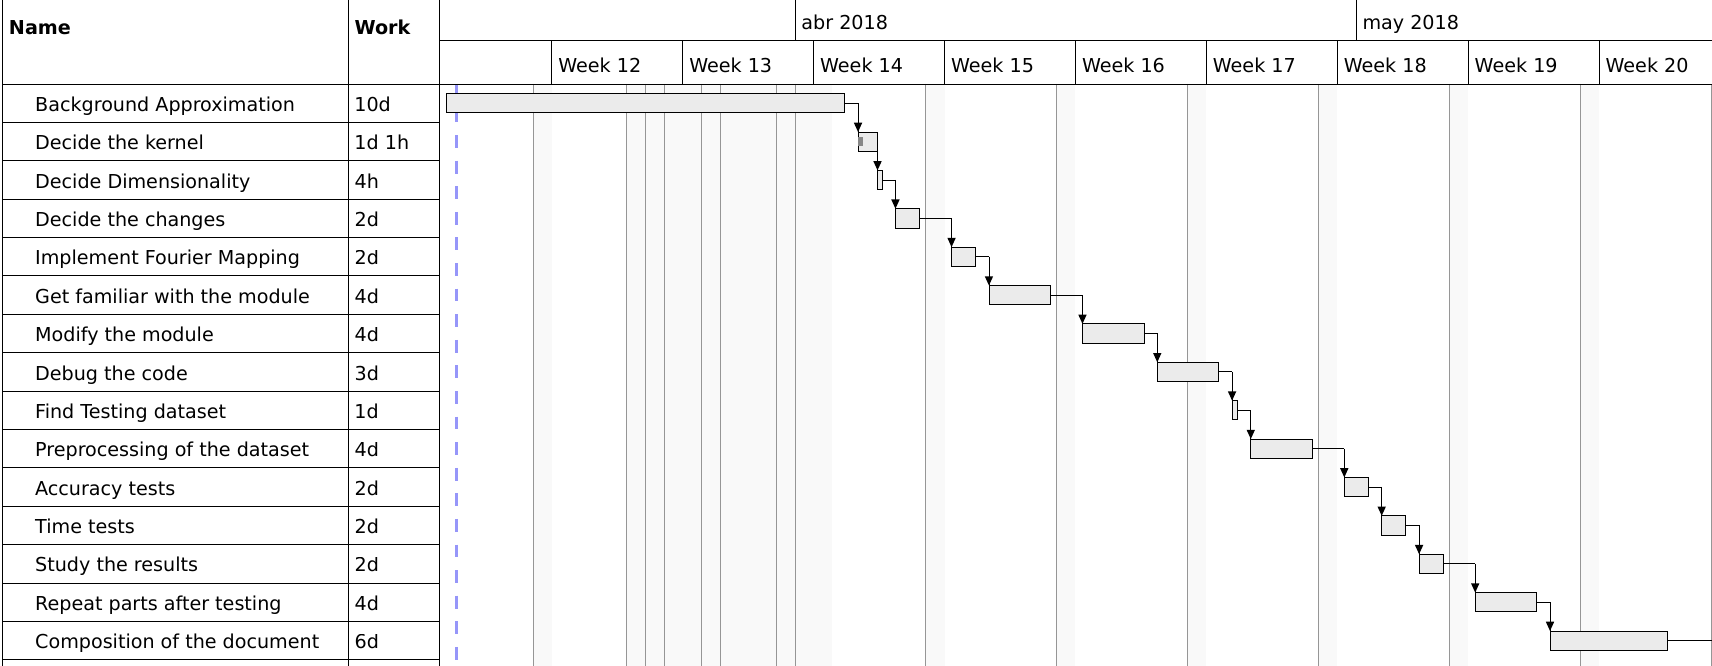
\includegraphics[width=\textwidth]{gant}
    \caption{Gantt chart of the whole project. The planning assumes 5 hours of work from Monday to Saturday and some rest during Holy Week}
    \end{figure}


    \begin{figure}[H]
    \centering
    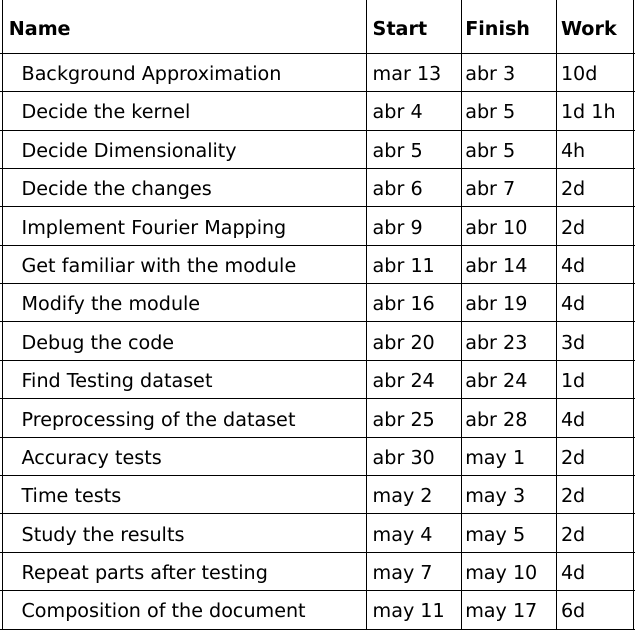
\includegraphics[width=\textwidth]{schedule}
    \caption{Schedule of the tasks}
    \end{figure}

    % 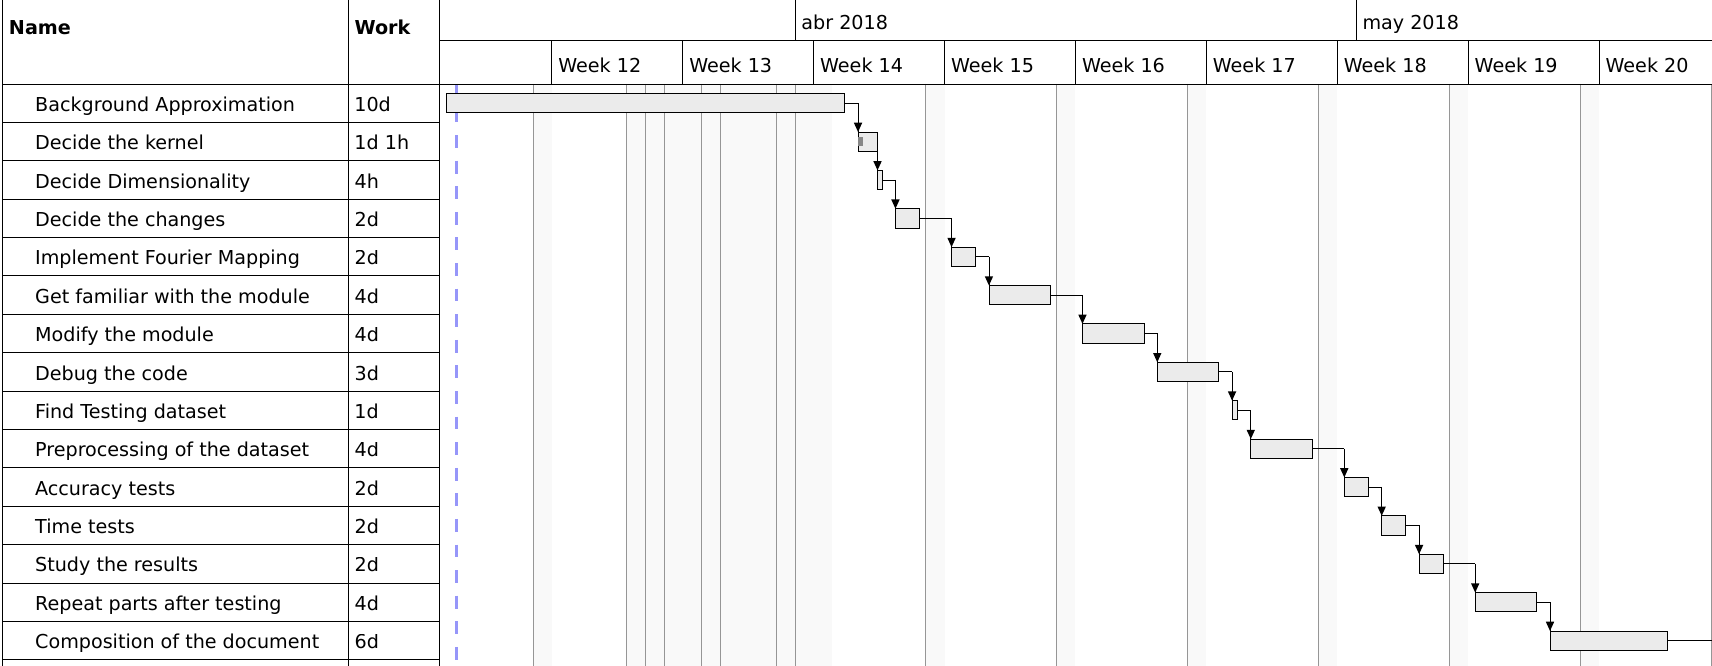
\includegraphics[width=\textwidth]{gant}


    % 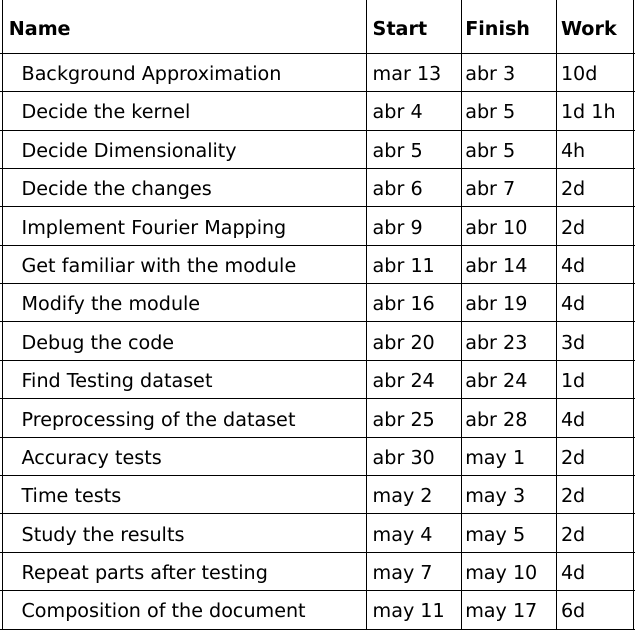
\includegraphics[width=\textwidth]{schedule}

    % Una vez tenga lo anterior debería ser fácil

    \section{Alternatives and action plan}

    As pointed out in the beggining of the document, the planning can be adapted from the initial one. As the Gantt chart shows, there are 4 weeks of margin from the scheduled end of the project and the deadline, so we have some flexibility. If a task task more than expected and there is not enough time, another task will have to be shortened.

    Here, some of the potential sources of delays are mentioned.

    \subsection{Complexity of the module}

    The Python 3 module from Scikit Project I plan to use may be too complicated to modify. I have planned much time in studying and modifying the code, but it could not be enough.

    \subsection{Bugs}

    I will certainly find bugs in my code. Detecting and correcting theme may be more laborious than expected, so it could delay the planning.




    % \section{Schedule}
    % \section{Project Planning}
    %
    %
    % \section{Action plan}
    % \section{Resources}






% \printbibliography


\end{document}
